\chapter{Experimental Evaluation}\label{chap:experiments}
This chapter will investigate the~performance of the~\emph{hybrid} approach for integrated synthesis methods extensions \,--\, multi-property and optimal synthesis \,--\, for various case studies and properties.
Moreover,~we will also introduce a~preliminary results of the~performance of the~designed approach for both \emph{parameter} and \emph{combined} synthesis.
Further on,~we demonstrate the~applicability of \toolname{} and interpret the~synthesis results for three of these case studies.
All experiments are run on a~Debian~GNU/Linux~10 machine with Intel(R) Core(TM) i7-3770K (8 cores at 3.50GHz) and using up to 32 GB RAM,~with all the~algorithms being executed single-threaded.

\section{Performance Evaluation of Advanced Methods}
This section aims to demonstrate the~performance of advanced integrated methods for both \textit{multi-property} and \textit{optimal} synthesis on various synthesis problems from different application domains.
In particular,~we compare its performance with the~\emph{one-by-one} enumeration representing the~baseline algorithm implemented in the~existing synthesis tools such as QFLan~\cite{qflan} and ProFeat~\cite{profeat}.
Experiments in previous papers~\cite{cegar,cegis} have shown that the~synthesis methods implemented in these tools have evident deficits on the~investigated benchmarks.
Moreover, experiments in~\cite{roman-DP} have shown that presented hybrid method significantly outperform both state-of-the art synthesis approaches \,--\, CEGIS and AR.
These facts is supported by comparing the~hybrid approach only with the~one-by-one enumeration we present in this section.
For each case study,~we report the~results for \textit{unfeasibility} problems with one property and two properties,~and \textit{optimal} synthesis problem and its \textit{relative} variant with $\varepsilon = 0.05$.
In all cases,~the~synthesis methods have to explore the~whole design space.
The~metrics marks with * represent the~qualified estimates.
We consider the following case studies:

\paragraph{Herman.}
This model represents distributed asynchronous protocol for rings with self-stabilisation~\cite{herman1,herman2}.
The~protocol is extended with a~choice for flipping several unfair coins,~and each station in the~ring includes one-bit memory.
All stations in the~ring have equivalent behaviour,~i.e.,~they are anonymous,~but they decide based on the~own local events and value of the~memory.
The~family maintains this anonymity and describes the~different variations of coin choice and updates of memory.
We are interested mainly in the~expected time until \emph{stabilisation}.
    
\begin{table}[h!]
\centering
\begin{tabular}{l|cccc}
    \hline \hline 
    & \multicolumn{1}{l}{\textbf{1 property}} & \multicolumn{1}{l}{\textbf{2 properties}} & \multicolumn{1}{l}{\textbf{optimal}} & \multicolumn{1}{l}{\textbf{$\mathbf{5\%}$-optimal}} \\ \hline
    \textbf{1-by-1} & 32h & 40h & 32h & \,--\, \\
    \textbf{Hybrid} & 90s & 105s & 21m & 8m \\ \hline \hline
\end{tabular}
\caption{\textbf{Herman}: Family size: $3.1M$, Number of parameters: $7$, Average MC size: $1.1k$.}
\end{table}

\paragraph{DPM.}
It represents a~partial information scheduler for a~disk power manager motivated by~\cite{dpm1}.
This model have been precise described in Section~\ref{sec:dpm}.
We are interested primarily in the~expected energy consumption and expected number of lost requests.

\begin{table}[h!]
\centering
\begin{tabular}{l|cccc}
    \hline \hline 
    & \multicolumn{1}{l}{\textbf{1 property}} & \multicolumn{1}{l}{\textbf{2 properties}} & \multicolumn{1}{l}{\textbf{optimal}} & \multicolumn{1}{l}{\textbf{$\mathbf{5\%}$-optimal}} \\ \hline
    \textbf{1-by-1} & 31d & 35d & 31d & \,--\, \\
    \textbf{Hybrid} & 72m & 84m & 9.7h & 6.2h \\ \hline \hline
\end{tabular}
\caption{\textbf{DPM}:  Family size: $43M$, Number of parameters: $16$, Average MC size: $3.6k$.}
\end{table}

\paragraph{Maze.}
It represents a planning problem typically modelled as POMDP~\cite{maze}.
The~family includes all deterministic strategies which are based on observation,~and containing small memory with a~fixed upper bound.
We are interested primarily in the~expected time to the \emph{goal}.

\begin{table}[h!]
\centering
\begin{tabular}{l|cccc}
    \hline \hline 
    & \multicolumn{1}{l}{\textbf{1 property}} & \multicolumn{1}{l}{\textbf{2 properties}} & \multicolumn{1}{l}{\textbf{optimal}} & \multicolumn{1}{l}{\textbf{$\mathbf{5\%}$-optimal}} \\ \hline
    \textbf{1-by-1} & 25h & 31h & 25h & \,--\, \\
    \textbf{Hybrid} & 63m & 65m & 78m & 59m \\ \hline \hline
\end{tabular}
\caption{\textbf{Maze}:  Family size: $9.4M$, Number of parameters: $22$, Average MC size: $0.2k$.}
\end{table}

\paragraph{Pole.}
It models balancing a pole in an unknown and noisy environment~\cite{pole}.
A~model controller optimises an~expected behaviour during the deployment without dependence on the~current (hidden) environment since it is preferred before the~finite set of environment behaviours.
The~family described schedulers that are independent of hidden information.
We are interested mainly in the~expected time until \emph{failure}.

\begin{table}[h!]
\centering
\begin{tabular}{l|cccc}
    \hline \hline 
    & \multicolumn{1}{l}{\textbf{1 property}} & \multicolumn{1}{l}{\textbf{2 properties}} & \multicolumn{1}{l}{\textbf{optimal}} & \multicolumn{1}{l}{\textbf{$\mathbf{5\%}$-optimal}} \\ \hline
    \textbf{1-by-1} & 23h & 30h & 23h & \,--\, \\
    \textbf{Hybrid} & 7s & 8s & 11m & 60s \\ \hline \hline
\end{tabular}
\caption{\textbf{Pole}:  Family size: $1.3M$, Number of parameters: $17$, Average MC size: $5.6k$.}
\end{table}

\paragraph{Grid.}
It represents a~model describing again partially observable MDPs (POMDPs)~\cite{pomdp1}.
There is an~agent who tries to locate a~target cell in a~4x4 grid.
We are interested in lower- and upper- bounded properties on the~expected number of steps.

\begin{table}[h!]
\centering
\begin{tabular}{l|cccc}
    \hline \hline 
    & \multicolumn{1}{l}{\textbf{1 property}} & \multicolumn{1}{l}{\textbf{2 properties}} & \multicolumn{1}{l}{\textbf{optimal}} & \multicolumn{1}{l}{\textbf{$\mathbf{5\%}$-optimal}} \\ \hline
    \textbf{1-by-1} & 16m & 19m & 16m & \,--\, \\
    \textbf{Hybrid} & 31s & 35s & 47s & 9s \\ \hline \hline
\end{tabular}
\caption{\textbf{Grid}: Family size: $65k$, Number of parameters: $8$, Average MC size: $1.2k$.}
\end{table}
    

\paragraph{Evaluation.}
As we have already said,~we are based on what has already been shown in previous articles~\cite{roman-DP,cegar,cegis}.
As a~basis,~we know that a~hybrid oracle is orders of magnitude faster than one-by-one enumeration when analysing single property.
Based on the~results obtained in the~framework of all considered case studies,~we can draw the~following conclusions,~which confirm the~tables above.
An~integrated \emph{multi-property} synthesis slows down both approaches,~although the~hybrid slowdown is almost negligible.
An~\emph{optimal} synthesis slows down only the~hybrid approach,~yet it is still incomparably faster than naive one-by-one enumeration.
Moreover,~a~hybrid oracle supports $\varepsilon$-optimal synthesis,~which is even faster.

\paragraph{\toolname{} scalability.}

\begin{table}[h!]
\centering
\begin{tabular} {l|c|c|c|c|c|c}
{\multirow{2}{*}{model}} & 1-by-1 & CEGIS & \multicolumn{2}{c|}{AR} & \multicolumn{2}{c}{\textbf{hybrid}} \\
& time & time & iters & time & (CEGIS,AR) iters & time \\
\hline
{\emph{Herman-5k}} & 1m & \textcolor{red}{$\geq$24h} & 531 & \textcolor{red}{3m} & (571, 7) & \textbf{12s} \\ \hline
{\emph{Herman-3M}} & 27h & \textcolor{red}{$\geq$48h} & 83k & \textcolor{red}{55h} & (16197, 3) & \textbf{17m} \\ \hline
\end{tabular}
\caption{Efficiency of synthesis methods for synthesising optimal \emph{Herman's stabilisation algorithm}.} 
\end{table}


\section{Performance Evaluation of Combined Synthesis}

\section{Applicability}

\paragraph{Maze.} This is a~planning problem typically considered as \textit{POMDP}.
This case-study is inspired by the~infamous cheese-maze example~\cite{maze}: a~simple maze where an~agent attempts to reach a~target location.
The family describes all \textit{MCs} by small-memory observation-based deterministic strategies (with a~fixed upper bound on the~memory).
We are interested in the~expected time to the~goal,~and therefore we use the~optimal synthesis to synthesize the~minimum.

\begin{figure}[ht!]
\centering
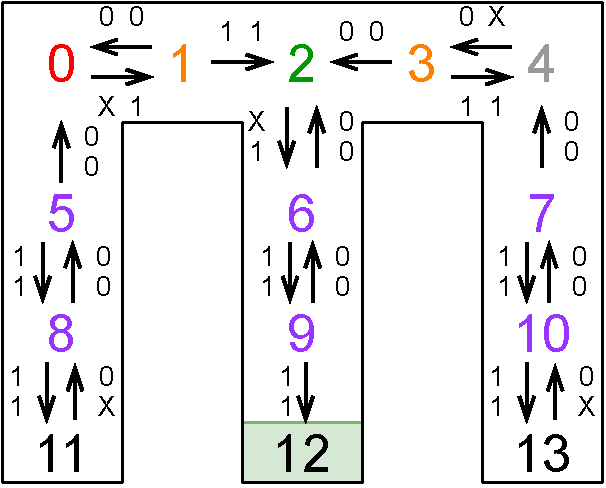
\includegraphics[width=0.4\textwidth]{figures/maze.pdf}
\caption{The state-space of the~\textit{Maze} model with a~marked target state and the~observation groups. A~right side represents the~found optimal strategy to reach the~target location within the~minimal expected time. The~initial state is selected randomly with a~memory value of 0.}%
\label{fig:maze}%
\end{figure}

The~state-space of the~model contains $13$ states and $1$ target state,~and we adapted this model as a~family with a~memory size of $1$ bit.
The~individual states are divided into $6$ different groups according to the~observation in which direction it is possible to go from a~given state.
The~next action is considered only according to the~current value of memory and the~observation group of the current state. 
Since we consider $6$ observation groups and $2$ possible memory values,~then the~model has $12$ possible configurations and $24$ holes because we have to determine the~new value of memory and the~direction from each configuration.
The~initial state is selected randomly with a~memory value of 0.
We want to synthesize the~\textit{reward} specification that reflects the~expected number of steps to reach the~target location: $\mathbb{R}\{steps\} = \, ? \; [\Diamond \, s=12]$.
As a~result of optimal synthesis,~the~minimum expected number of steps is equal to $9.8367$.
The~obtained synthesized strategy corresponds to human intuition and ensures direction always to the~target state,~with a~few exceptions at initial states,~e.g.,~initial configuration $(10, 0)$.
This deficiency is caused by the~fixed upper bound on the~memory,~and therefore it can be easily suppressed by raising the~possible values of memory to $3$.
In more precise, the strategy tries to choose from the current state the direction, which decrease the distance to the target location.
Moreover, it uses the memory to distinguish the different choices of directions from the states in the same observation group.
In this minimal synthesis was explored the family about size $9437184$ with $22$ holes, and the analysis taken $33$ CEGAR iterations and $43343$ CEGIS iterations, where were analyzed the models with average size $473$ at MDP, respectively $323$ at DTMC.
The overall run-time of the analysis was $36.82$ minutes.


\paragraph{Herman.}
This self-stabilisation algorithm provides a~simple randomised solution to recovering from faults in~an N-process token ring~\cite{herman-1,herman-2}.
At every step of the~algorithm,~each process with a~token decides whether to keep it or pass it on to its left neighbour,~with the~decision being based on the~outcome of a~random coin toss.
The~protocol is extended with a~bit of memory for each process in the~ring,~and the~choice to flip various unfair coins.
Nodes in the~ring are anonymous,~they all behave equivalently,~but may change their local memory based on local events.
The~family describes variations of memory-updates and coin-selection,~but always preserves anonymity.

Since $N$ must be odd,~we constructed a~network of $5$ identical processes in a~ring.
We are interested in the~expected amount of time required for algorithm execution,~i.e.,~the expected number of steps needed until stabilisation occurs:~$\mathbb{R}\{steps\} = \, ? \; [\Diamond \, num\_tokens=1]$.
We research how the~algorithm performance varies for different probability distributions of $\mathit{p}$, used to randomise processes' choices at each step. 
Since we consider the~boolean variable and $\mathit{1}$-bit memory for each process,~the number of possible configurations at each step is $4$.
We consider the~individual distribution of $\mathit{p}$ for each configuration,~the~new memory values for both decisions when the~process has token,~and also new memory value when it has not token \,--\, $7$ synthesised holes.
We decided to research $24$ different values of the~probability $\mathit{p} \in \{0.02, 0.04 \dots, 0.50 \}$, resulting in a~family of size $3125000$.
The~result of minimal synthesis shows that for $N=5$ is the~optimal setting $\mathit{p=0.5}$ for all synthesised distributions.
When the~process passes the~token,~it sets its own local memory to $1$,~otherwise;~it sets it to $0$.
Since the~memory contains $1$ only after the~token is passed,~when the~process variable is equal to $0$,~the~configuration $(1, 1)$ can never occur.
Therefore,~the~synthesis can terminate with an~arbitrary probability distribution for relevant hole without affecting the~minimal expected time.
We can conclude, that with a sufficiently small number of processes is the best strategy usage the fair coin for randomising choices.

\paragraph{Pole.}
This benchmark considers a~balancing pole in an~unknown and noisy environment~\,--\,~motivated by~\cite{pole-1,pole-2}.
At deploy time,~the controller should optimize the~expected behaviour without depending on the~actual (hidden) environment,~because of higher priority than a~finite set of environment behaviours.
Therefore,~the~family describes schedulers that do not depend on confidential information.
We are interested in the~expected time until \textit{failure}.

The~state space is designed as 2D-space,~where both coordinates have the~same dimension~\,--\,~in our experiments was set to $7$.
Since the~scheduler has to determine the~direction within inner positions of the~space ($5\times5$),we consider $25$ possible holes.
We allow only the~directions for each possible configuration that maintain the~pole in the required balance.
For some configurations,~we set the~constant direction,~and therefore the~total size of the~family is $1327104$.
We synthesised the~minimum and maximum expected time until failure with the~following reward specification:~$\mathbb{R}\{rounds\} = \, ? \; [\Diamond \, x = 0 \, \lvert \, y = 0 \, \lvert \, x = 7 \, \lvert \, y = 7]$.
The~minimal synthesis terminates with the~result of $7.89$ within $6$ minutes and the~following strategy.
In the~given configuration,~the~scheduler always selects such a~possible action that deflects the~pole as much as possible.
In other words,~the~scheduler tries to move around the~perimeter of the~interior space,~i.e.,~in the~positions from which a~terminate configuration can be reached in one action.
On the contrary,~the~scheduler representing the~strategy which corresponds to the~maximal time behaves asymmetrically.
It always selects an~action that changes the~position as close as possible to the~centre of the~entire 2D-space,~that is,~as far as possible from the~positions that are close to the~terminate configurations.
The~maximum synthesis took $9.5$ minutes,~and the~result was set at $16.66$.
We can conclude,~that both synthesises strategies were derived concern to given specifications correctly.
The~model checking within these analysis processed over the~MDP in the~average of size $6825$ and DTMC in the~average size of $6457$.
The~minimal synthesis takes 2189 CEGAR and 3463 CEGIS iterations,~and maximal 3491 and 5573 iterations respectively.

